
\subsubsection{Robust model fitting--RANSAC}
To perform the image stitching in the section above, we had to find the homography parameters that best described the transformation from one image to another. Because the detection of the feature points can be noisy, the homography fitting needs to be robust against inevitable feature mis-matches between images.  A good algorithm to fit models to data robustly is  RANSAC \cite{Fischler1981}, which stands for RANdom SAmpling with Concensus.  Introduced in 1981, it has been a workhorse in computer vision over the years since \cite{Zisserman2006}.

The procedure for RANSAC is simple, and the name contains most of the steps of the algorithm.  First, RANdomly select a sufficient set of datapoints to fit the parameters of some model.  The could be the parameters that define a line, some other structure, or a homography.  Then, compute the model parameters from the randomly SAMpled set of points. Compute the inliers in the dataset--the datapoints that fit the model (or achieve Consensus) to within some tolerance.  Repeat that procedure some number of times, $N$.    Compute a final model from the set of inlier points corresponding to the largest number of inlier datapoints.

Figure~\ref{fig:ransac} shows a simple instantiation of this algorithm for the case of robustly fitting a straight line model to a collection of datapoints, Fig.~\ref{fig:ransac}~(a).  First, a number of datapoints, sufficient to uniquely specify the model parameters, are drawn from the dataset.  For this problem, that is two points.  Two randomly selected points are marked in green in Fig.~\ref{fig:ransac}~(b).  After finding the line that passes through those two points, the number of "inliers"--datapoints within $\epsilon$ of the model--is determined.  For the line of (b), the number of inliers is three. This process is repeated until some desired number of samplings, $S$, have been drawn.  The output model is fitted from all the inlier datapoints corresponding to the model that led to the most inlier datapoints.

The authors derive a heuristic for the number of samples, $S$, required to be assured a good model fit.  Let $n$ be the number of datapoints required to specify the model, and let $w$ be (an estimate of) the probability that any selected datapoint is within the error tolerance of the model.   For the example of Fig.~\ref{fig:ransac}, as seen in (f), there are $n=2$ outliers out of 11 points, so $w = 0.18$ (in general, this value needs to be estimated).  $w^n$ is the probability that all the selected points are inliers, and $1 -  w^n$ is the probability that at least one selected point is an outlier.  The probability that in k trials only bad models are selected is then $(1 -  w^n)^k$.  If $p$ is the probability of selecting the correct model, we have (see also \cite{wikiRANSAC}
\begin{equation}
    1-p = (1 -  w^n)^k
\end{equation}
Taking the logarithm of both sides lets us solve for $k$, the number of RANSAC iterations required to find a good fit, with probability $p$:
\begin{equation}
        k = \frac{\log(1-p)}{\log(1-w^n)}
        \label{eq:k}
\end{equation}
For the example of Fig.~\ref{fig:ransac}, for 95\% accuracy, $k = \frac{\log(-05)}{\log(1-0.18^2)} = \frac{-1.3}{-0.0143} = 91$
So with 91 trials, we would have 95\% confidence of finding the correct model through RANSAC. 


\begin{figure}
\centerline{
\sublabel{a}{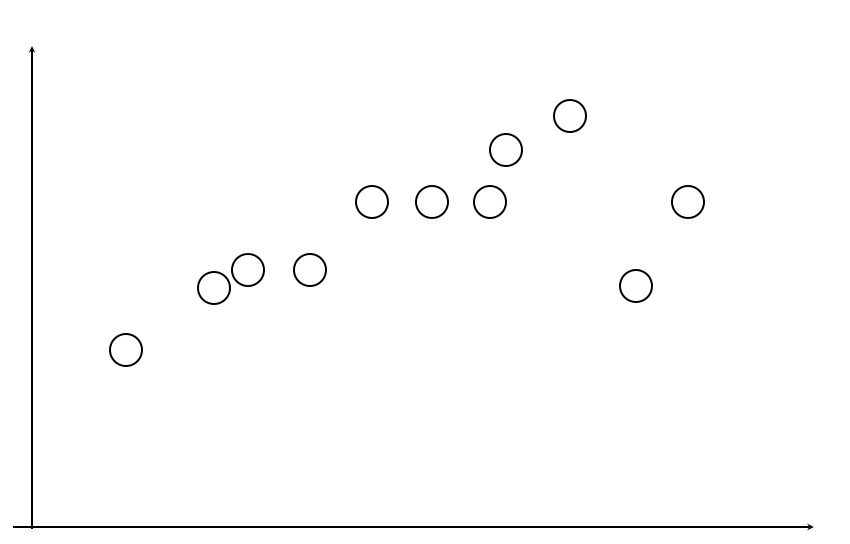
\includegraphics[width=0.4\linewidth]{figures/stereo/ransac1.jpg}}
\sublabel{b}{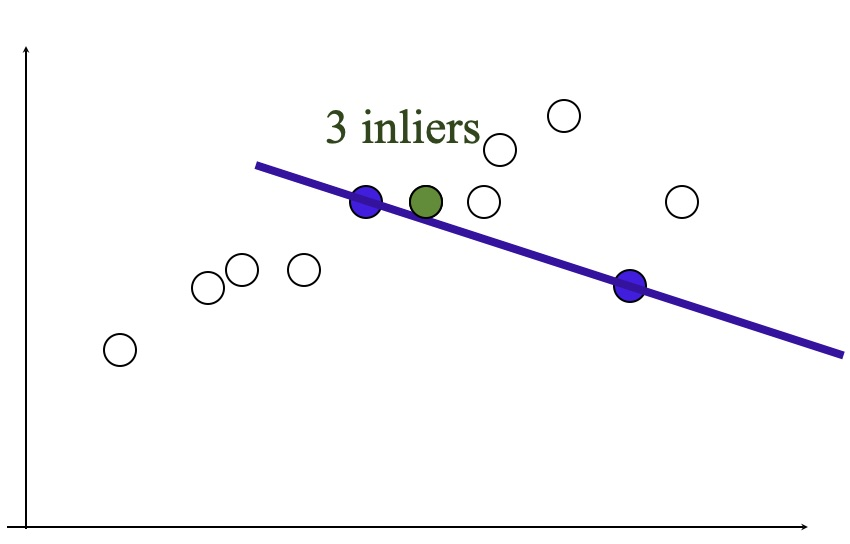
\includegraphics[width=0.4\linewidth]{figures/stereo/ransac2.jpg}}}
\centerline{
\sublabel{c}{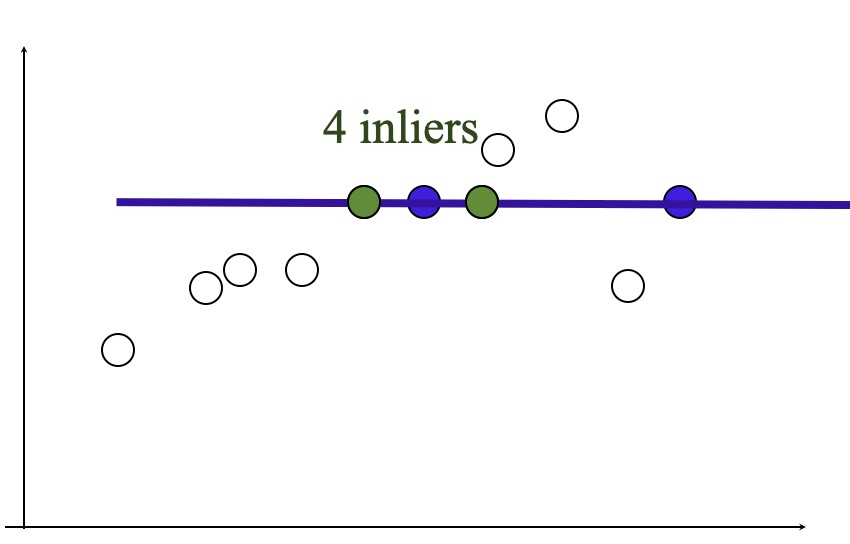
\includegraphics[width=0.4\linewidth]{figures/stereo/ransac3.jpg}}
\sublabel{d}{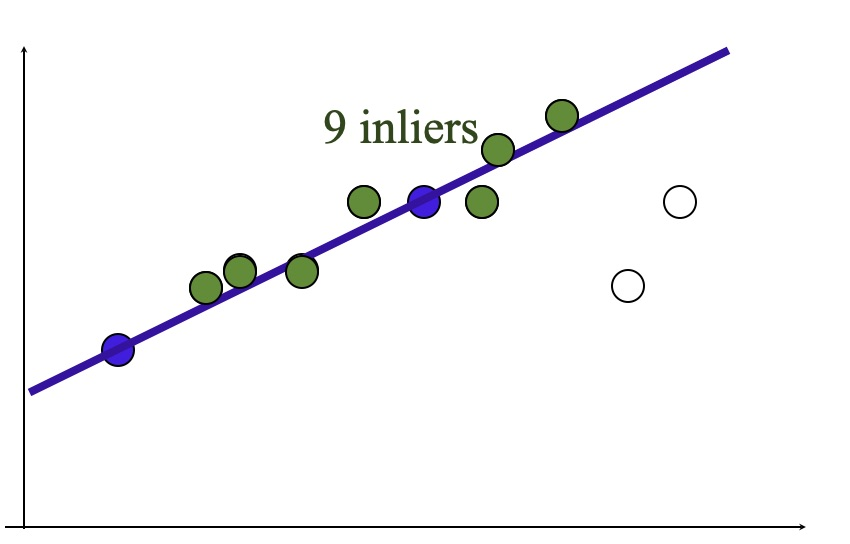
\includegraphics[width=0.4\linewidth]{figures/stereo/ransac4.jpg}}}
\centerline{
\sublabel{e}{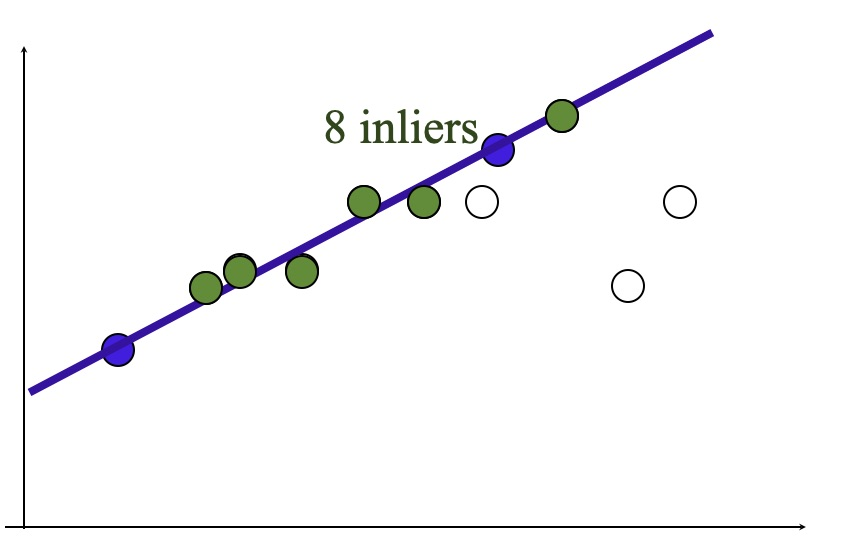
\includegraphics[width=0.4\linewidth]{figures/stereo/ransac5.jpg}}
\sublabel{f}{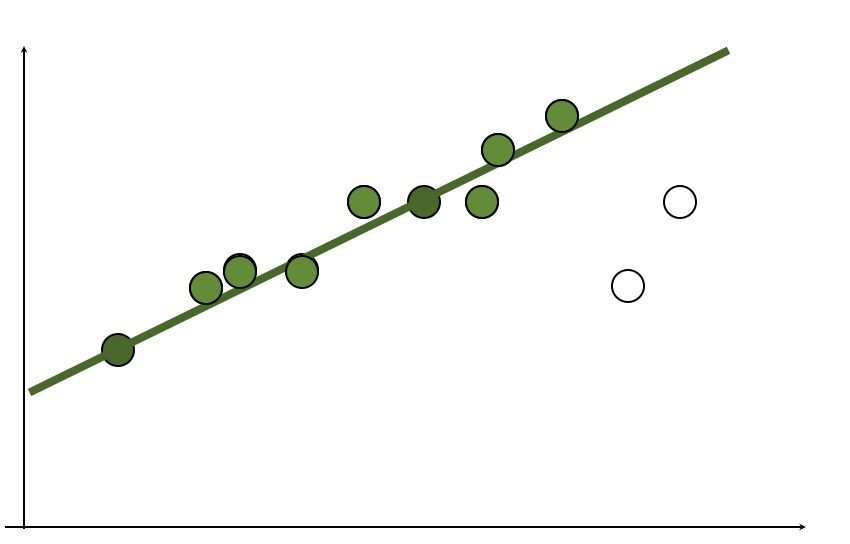
\includegraphics[width=0.4\linewidth]{figures/stereo/ransac6.jpg}}}
\caption{RANSAC applied to robust estimation of line parameters. (a) datapoints for which robust line estimation is sought. (b) two points (in blue) are selected at random, sufficient to estimate line model parameters. The number of inliers is computed for this model. (c) - (e) repeat k times. (f) select the model with the maximum number of inliers.}
\label{fig:ransac}
\end{figure}

